% Setup - do not change
\documentclass[11pt]{article}
\usepackage[english]{babel}
\usepackage[utf8]{inputenc}
\usepackage[toc,page]{appendix}
\usepackage{amsmath,amsthm,amssymb,graphicx,pdfpages,lipsum,hyperref, wrapfig}
\usepackage[none]{hyphenat}
\setlength\parindent{0pt}
\usepackage[top=0.9in, left=0.9in, bottom=0.9in, right=0.9in]{geometry} 
%%%%%%%%%%%%%%%%%%%%%%%%%%%%%%%%%%%%%%%%%%%%%%%%%%%%%%%%%%%%%%%%%%%
% add other packages here if required


%%%%%%%%%%%%%%%%%%%%%%%%%%%%%%%%%%%%%%%%%%%%%%%%%%%%%%%%%%%%%%%%%%% the '%' symbol denotes comments

% Begin document creation
% DELETE THE \lipsum PLACEHOLDERS WHEN YOU BEGIN
\title{\textbf{Can AirBnB Data Enhance Taxi Ride Profitability Classification?}}
\author{Declan Jackson \\
        Student ID: 1080086}

\begin{document}
\maketitle

\section{Introduction}
\subsection{Background Information}
% Link to a 30 min tutorial if you require revision: https://www.overleaf.com/learn/latex/Learn_LaTeX_in_30_minutes
In a buzzing metropolis such as New York City, an understanding of transport activity and spending is forever sought after. Ever since the release of the New York Taxi and Limousine Commission’s Trip Record Data, as part of the NYC Open Data Project \cite{open_data_website}, many analyses have been carried out to investigate taxi demand \cite{taxi_demand}, supply \cite{taxi_supply}, and revenue \cite{taxi_revenue}. This report however, sets out to investigate spending through both taxi trip data, and accommodation listing data from rental company AirBnB. Through such analysis, the report aims to determine whether it would be profitable for taxi companies and green and yellow taxi drivers to purchase AirBnB data to improve the classification of ride profitability. 

\subsection{The Data}
\subsubsection{AirBnB Dataset}
The AirBnb data from this analysis was sourced from Inside AirBnB \cite{airbnb_data} and covers all the listings in New York city, with their location, description, and other metrics. It contains data about listings from 2019, with the last recorded review date in the data being in July. The data set covers around 50’000 listings, with 15 different metrics from each listing.

\subsubsection{NYC TLC Dataset}
The taxi data was sourced from the New York Taxi and Limousine Commission (‘TLC’) Trip Record database \cite{taxi_data}, from May 2019 to July 2019. These dates were chosen since they lined up most accurately with the AirBnB data. Furthermore, this time was the busiest for NYC in terms of tourism \cite{tourism_data}and is therefore the most appropriate to use in conjunction with AirBnB data. The three months of data records approximately 22 million trips, with each trip having 18 different features.

Yellow and green taxis will be studied in this report. This is because the area covered is much greater than just yellow taxis, which therefore broadens the applications of our model. For-Hire-Vehicles were not considered as fare amount data was not included in their data set. 

\subsubsection{NYC TLC Taxi Zone Dataset}
Geographical data was also sourced from TLC \cite{geo_data}, outlining the taxi zones used to describe each trip’s pick up and drop off point. There are 263 valid zones. 

\subsection{Chosen Attributes}
The attribute that is being classified in our machine learning model is trip profitability (see equation 1). Our model will classify a trip’s profitability based on driving factors and factors from the AirBnB data. 

The driving factors are as follows:
\begin{itemize} 
    \item The duration of the trip
    \item The hour in which the passenger is going to be picked up for the trip
    \item The probability of the given trip being requested
    \item The probability of finding a trip in the zone in which you drop off the passenger
    \item The borough from which the passenger is picked up
    \item The borough at which the passenger is dropped off

\end{itemize} 

The duration of a trip will not be known exactly by a driver when classifying possible trip profitability prior to a trip. For the purpose of this model, we are assuming that taxi drivers can predict trip duration. 
Each trip will also be classified using AirBnB metrics from the listings in the trip pick up zone and drop off zone. These metrics are: 
\begin{itemize} 
    \item Number of zone listings 
    \item Median listing price
    \item Median number of minimum nights of a listing
    \item Median number of reviews
    \item Median number of reviews per month
\end{itemize} 


\section{Metrics}

\subsection{Trip Profitability Rate}
When calculating the profitability of a given ride we need to consider three factors:
\begin{enumerate} 
    \item The difference in the fare amount and the resource cost of the trip
    \item How likely a trip from that zone at that hour is (e.g. a singular long trip far away from the city at an odd hour may be profitable, but this does not mean there will always be profitable rides in that area) 
    \item The taxi demand in that zone, at that hour (e.g. a trip is not profitable if the next pick up destination is far away)
\end{enumerate}

Combining these factors, the following equation was used to calculate the profitability \emph{P}, of a given ride \emph{r}, going from a given zone \emph{$Z_a$} to a given zone \emph{$Z_b$} at time \emph{t}:

\begin{equation}
    P_r = \mathbf{E}(ZD_{a,t1}) \times \frac{60 * (Trip fare - CPM * Trip Distance)}{Trip Duration} \times  \mathbf{E}(ZD_{b,t2})
\end{equation}

Where CPM (Driving Cost Per Mile) = \$0.58, as defined by the IRS \cite{IRS}, and the expected Zone Demand of a given zone \emph{Z}, at time \emph{T} is given by:

\begin{equation}
    \mathbf{E}(ZD_{Z,T}) = \frac{\sum_{z=Z, t=T}Trip_{z,t}}{\sum_{d \in D} d}
\end{equation}

And d $\in$ D are the days in the given dataset

% You can have \section{}, \subsection{}, and \subsubsection{}
\section{Preprocessing}
\subsection{NYC TLC Dataset}
The pre-processing steps for the taxi data were as follows:
\begin{enumerate} 
    \item Only take trips with a valid Vendor ID (either 1 or 2)
    \item Drop trips completed before May 1 2019, and trips started after June 30 2019
    \item Drop trips with negative trip distance, and trips with a distance in the top 0.1\% to ensure the classifier does not learn on outliers (see figure 1)
    \item Only take trips with a RateCodeID equal to 1 or 2. This is because negotiated fairs/group rides are harder to predict, and should not be a factor in predicting profitability. Secondly, trips to/from Newark, Nassau, or Westchester are not considered due to their rarity in comparison to standard/JFK trips
    \item Only take trips with a valid \verb|PULocation| and \verb|DOLocation| (1 to 263)
    \item Drop all trips with negative fare. This is because these trips will skew profitability, and predicting negative fare rides is not the focus of this report
    \item Only take trips paid with credit card avoid learning on outliers (e.g. ‘Dispute’ or ‘No charge’) and to ensure accuracy of tip data, as tips are only recorded for credit card payments
    \item Create column \verb|trip_duration| from finding the difference in pick up and drop off times 
    \item Remove trips longer than 2.5 hours as they are outliers (see figure 2)
    \item Create columns \verb|pu_hour| and \verb|do_hour|, corresponding to the hours in which the passenger is picked up and dropped off
    \item Create columns \verb|pu_zone_hourly_demand| and \verb|do_zone_hourly_demand| according to the equation (2)
    \item Create column \verb|trip_profit_rate| according to equation (1)
    \item Create column \verb|profit_label| according to the bin the trip’s profit rate belongs to. The profit rates are placed into three equal frequency bins of low, medium and high profitability (labelled 1, 2, and 3 respectively)
\end{enumerate}
The final dataset contained approximately 14 million rows, with each trip having 14 different features. Choosing credit card trips was the most notable cause of reduction, reducing the data set by 29\%.
\begin{figure}[ht]
\centering
\begin{minipage}[b]{0.45\linewidth}
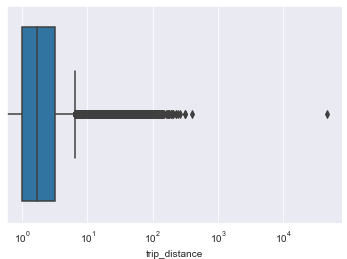
\includegraphics[scale=0.6]{plots/distance_pre_box.png}
\caption{Distribution of trip distance before cleaning}
\label{fig:minipage1}
\end{minipage}
\quad
\begin{minipage}[b]{0.45\linewidth}
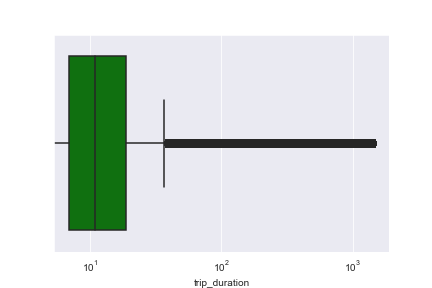
\includegraphics[scale=0.6]{plots/duration_pre_box.PNG}
\caption{Distribution of trip duration before cleaning}
\label{fig:minipage2}
\end{minipage}
\end{figure}


 \subsection{AirBnB Dataset}
 The pre-processing steps for the AirBnB data were as follows:
 \begin{enumerate} 
    \item Create column \verb|ABLocationID| by assigning every listing with a taxi zone location according to the TLC Taxi Zone shapefile \cite{geo_data}
    \item Fill missing values in \verb|reviews_per_month| with 0
    \item Round values in \verb|minimum_nights| to the nearest integer
    \item Group the data set by \verb|ABLocationID|, to obtain number of listings per zone, and other metrics as specified in section 1.3
\end{enumerate}

The final data set contained 242 rows, each corresponding to a specific zone (not all zones contained AirBnB listings). Each zone had 6 features.

\section{Preliminary Analysis - Factors Affecting the Model}
\subsection{Time of Pick Up}
The first variable effecting the profitability of a ride, is the time that the passenger is picked up. We can see that this data has two major peaks around 8:00am and 5:00pm - 7:00pm, most likely the times at which civilians are going to or coming from work. Trip demand may be higher at these times, and therefore trips may be more profitable as taxi drivers would not have to wait as long (i.e. Zone Hourly Demand is higher)

\subsection{Trip Duration}
The distribution of trip profitability, on a log scale, looks to be right skewed. This is due to the high volume of short taxi trips, most likely in the Manhattan. This may cause the model to predict better on trips which have a lower trip distance, as opposed to longer trips. 

\begin{figure}[ht]
\centering
\begin{minipage}[b]{0.45\linewidth}
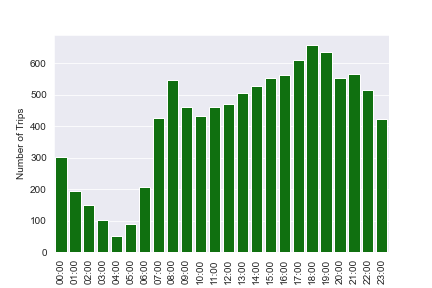
\includegraphics[scale=0.6]{plots/pickup_time.png}
\caption{Distribution of trip pick up times}
\label{fig:minipage1}
\end{minipage}
\quad
\begin{minipage}[b]{0.45\linewidth}
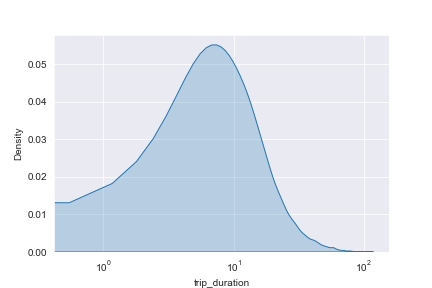
\includegraphics[scale=0.6]{plots/trip_duration.png}
\caption{Distribution of trip duration}
\label{fig:minipage2}
\end{minipage}
\end{figure}

\begin{figure}[!htb]
\centering
\begin{minipage}[b]{0.45\linewidth}
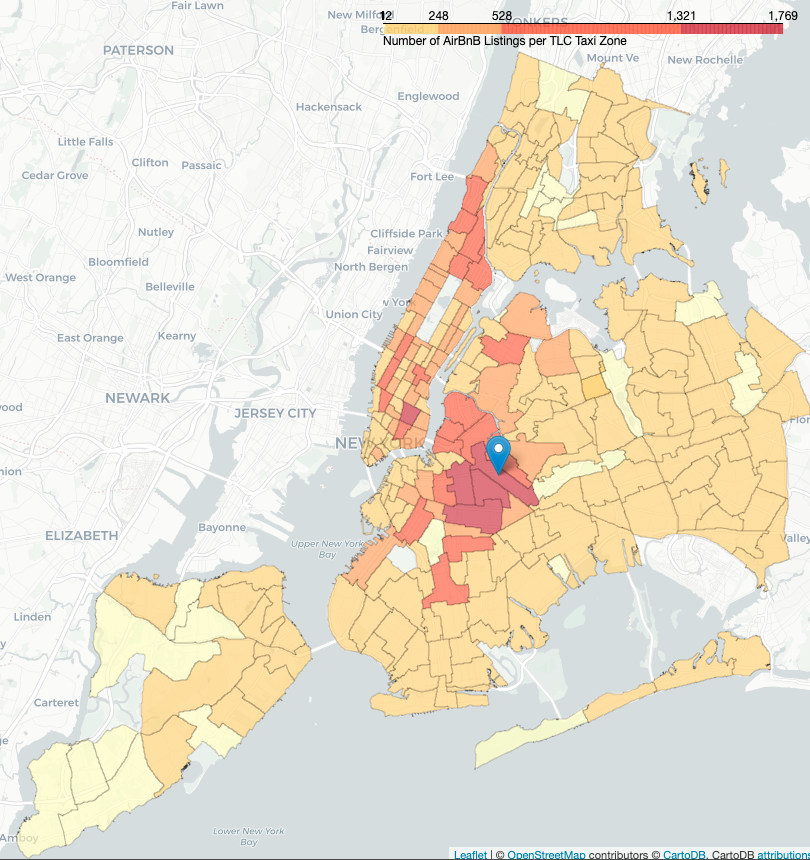
\includegraphics[scale=0.26]{plots/num_listings.png}
\caption{Choropleth map of the number of listings per NYC Taxi Zone}
\label{fig:minipage1}
\end{minipage}
\quad
\begin{minipage}[b]{0.45\linewidth}
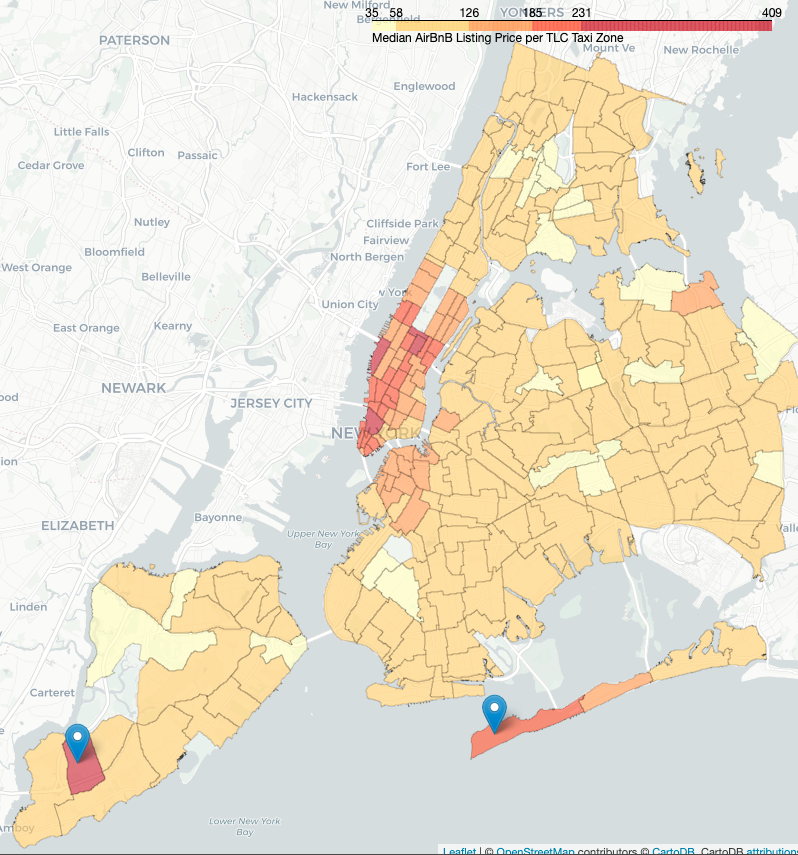
\includegraphics[scale=0.26]{plots/median_prce.png}
\caption{Choropleth map of the median price of listings per NYC Taxi Zone}
\label{fig:minipage2}
\end{minipage}
\end{figure}

\subsection{Number of Listings and Median Price}
The number of listings per taxi zone (Figure 5) may effect how many tourists visit that area, or how many AirBnB residents (who are not likely to have access to a car) will need rides from that zone. In Figure 5 we see the popular areas are around Brooklyn, with the most listing-dense zone being Bushwick South (see marker), having 1769 AirBnB listings. From the Figure 6 we can see that that southern Manhattan, as well as the zones Rossville/Woodrow (left marker) and Breezy Point/Fort Tilden/Riis Beach (right marker) have a high median price for their listings. The more expensive AirBnb zones may attract more wealthy travellers, which in turn could increase profitability of a given trip, as the passenger more likely to tip well or be more willing to travel further distances.

\subsection{Trip Profitability by Zone}
Central Manhattan seems to have the highest average profitability label for trips both starting (Figure 7) and finishing there (Figure 8). This draws some similarities to the median price choropleth map. Unlike number of listings, which has its most dense point in Brooklyn, a trip's profitability label is most likely going to be 1 (low) unless a trip begins or starts in Manhattan or near JFK airport. Reflecting Figures 7 and 8, the overwhelming majority of trips start and end in Manhattan (see Figure 9), which makes it clear - the majority of taxi business and profitability lies in Manhattan. Excluding Manhattan to Manhattan trips however (Figure 10), we see that many rides start and finish in Queens and Brooklyn, the most popular areas for AirBnB listings (Figure 5). Such visual evidence is not supported by Figure 11 however, where we see that our goal attribute, \verb|profit_label|, is not strongly correlated with any of the attributes under investigation. This suggests that perhaps the AirBnB data will not assit our profitability classifier. It is interesting to note however the two attributes most strongly correlated with the label, \verb|DO_price| and \verb|trip_duration|. The negative correlation of trip duration suggests that shorter rides are more profitable, most likely due to the \$2.50 initial charge \cite{taxi_fare} outweighing any small driving costs. The correlation with \verb|DO_price| is also interesting - trips ending in zones with more expensive AirBnB listings tend to be more profitable.


\begin{figure}[!htb]
\centering
\begin{minipage}[b]{0.45\linewidth}
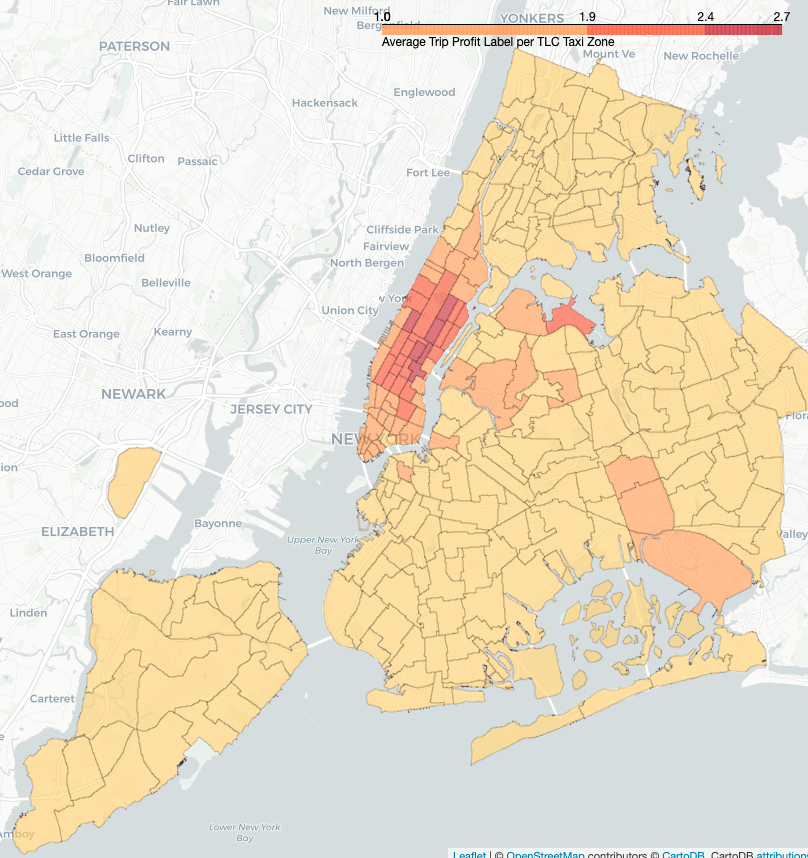
\includegraphics[scale=0.23]{plots/pu_profit.png}
\caption{Average profitability label of trips starting in a given zone}
\label{fig:minipage1}
\end{minipage}
\quad
\begin{minipage}[b]{0.45\linewidth}
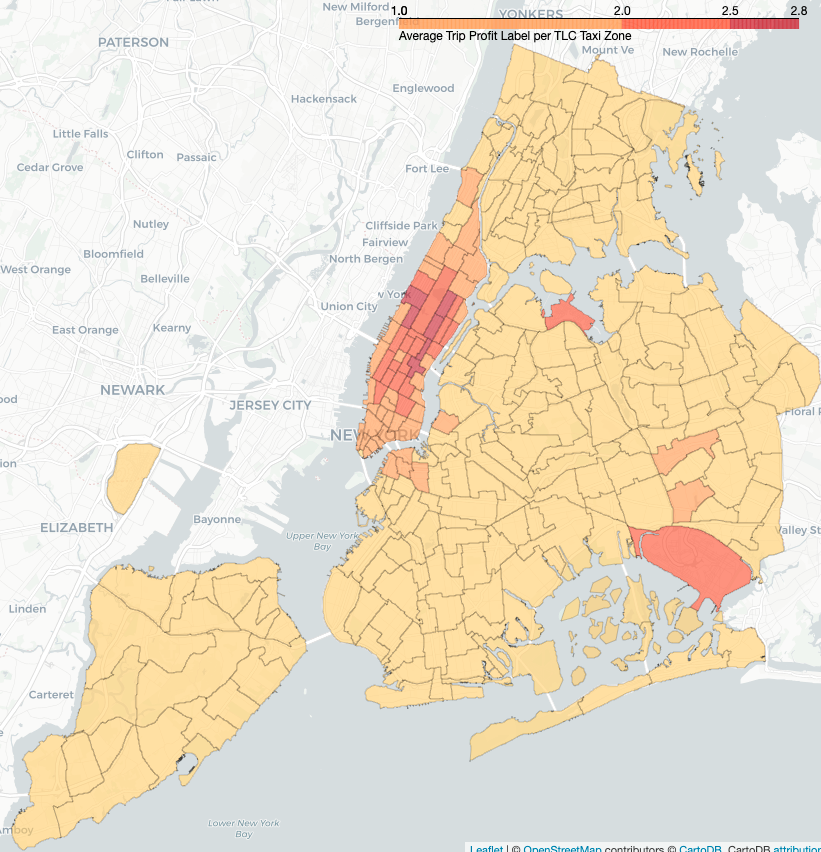
\includegraphics[scale=0.23]{plots/do_profit.png}
\caption{Average profitability label of trips finishing in a given zone}
\label{fig:minipage2}
\end{minipage}
\end{figure}

\begin{figure}[hbt!]
 \centering
 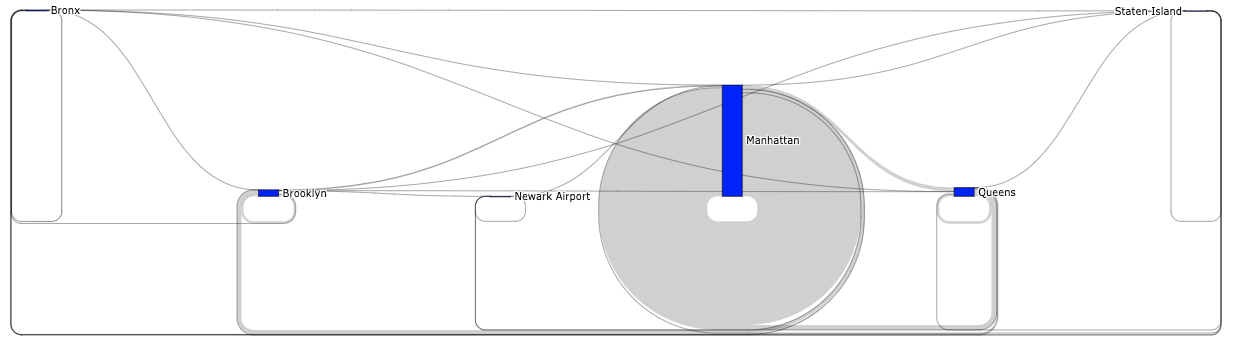
\includegraphics[scale=0.4]{plots/sankey.png}
 \caption{Sankey diagram summarising the movement of taxis between boroughs}
\end{figure}

\begin{figure}[hbt!]
 \centering
 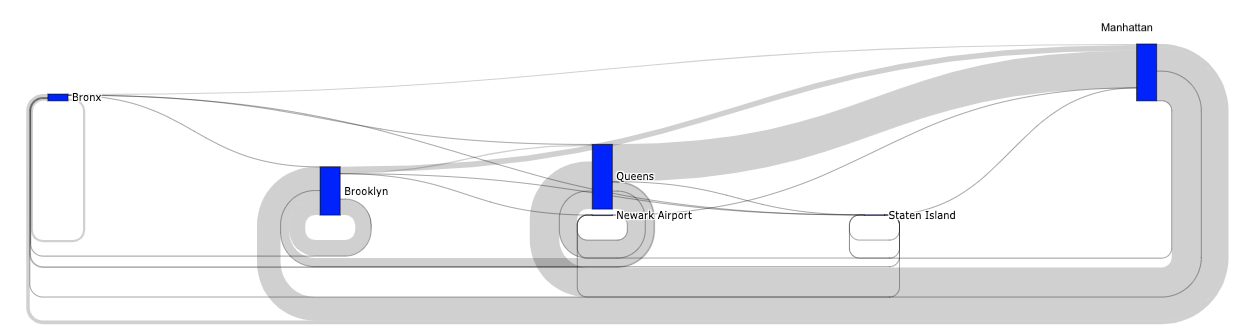
\includegraphics[scale=0.42]{plots/sankey_exc.png}
 \caption{Sankey diagram excluding trips which start and end in Manhattan}
\end{figure}


\begin{figure}[hbt!]
 \centering
 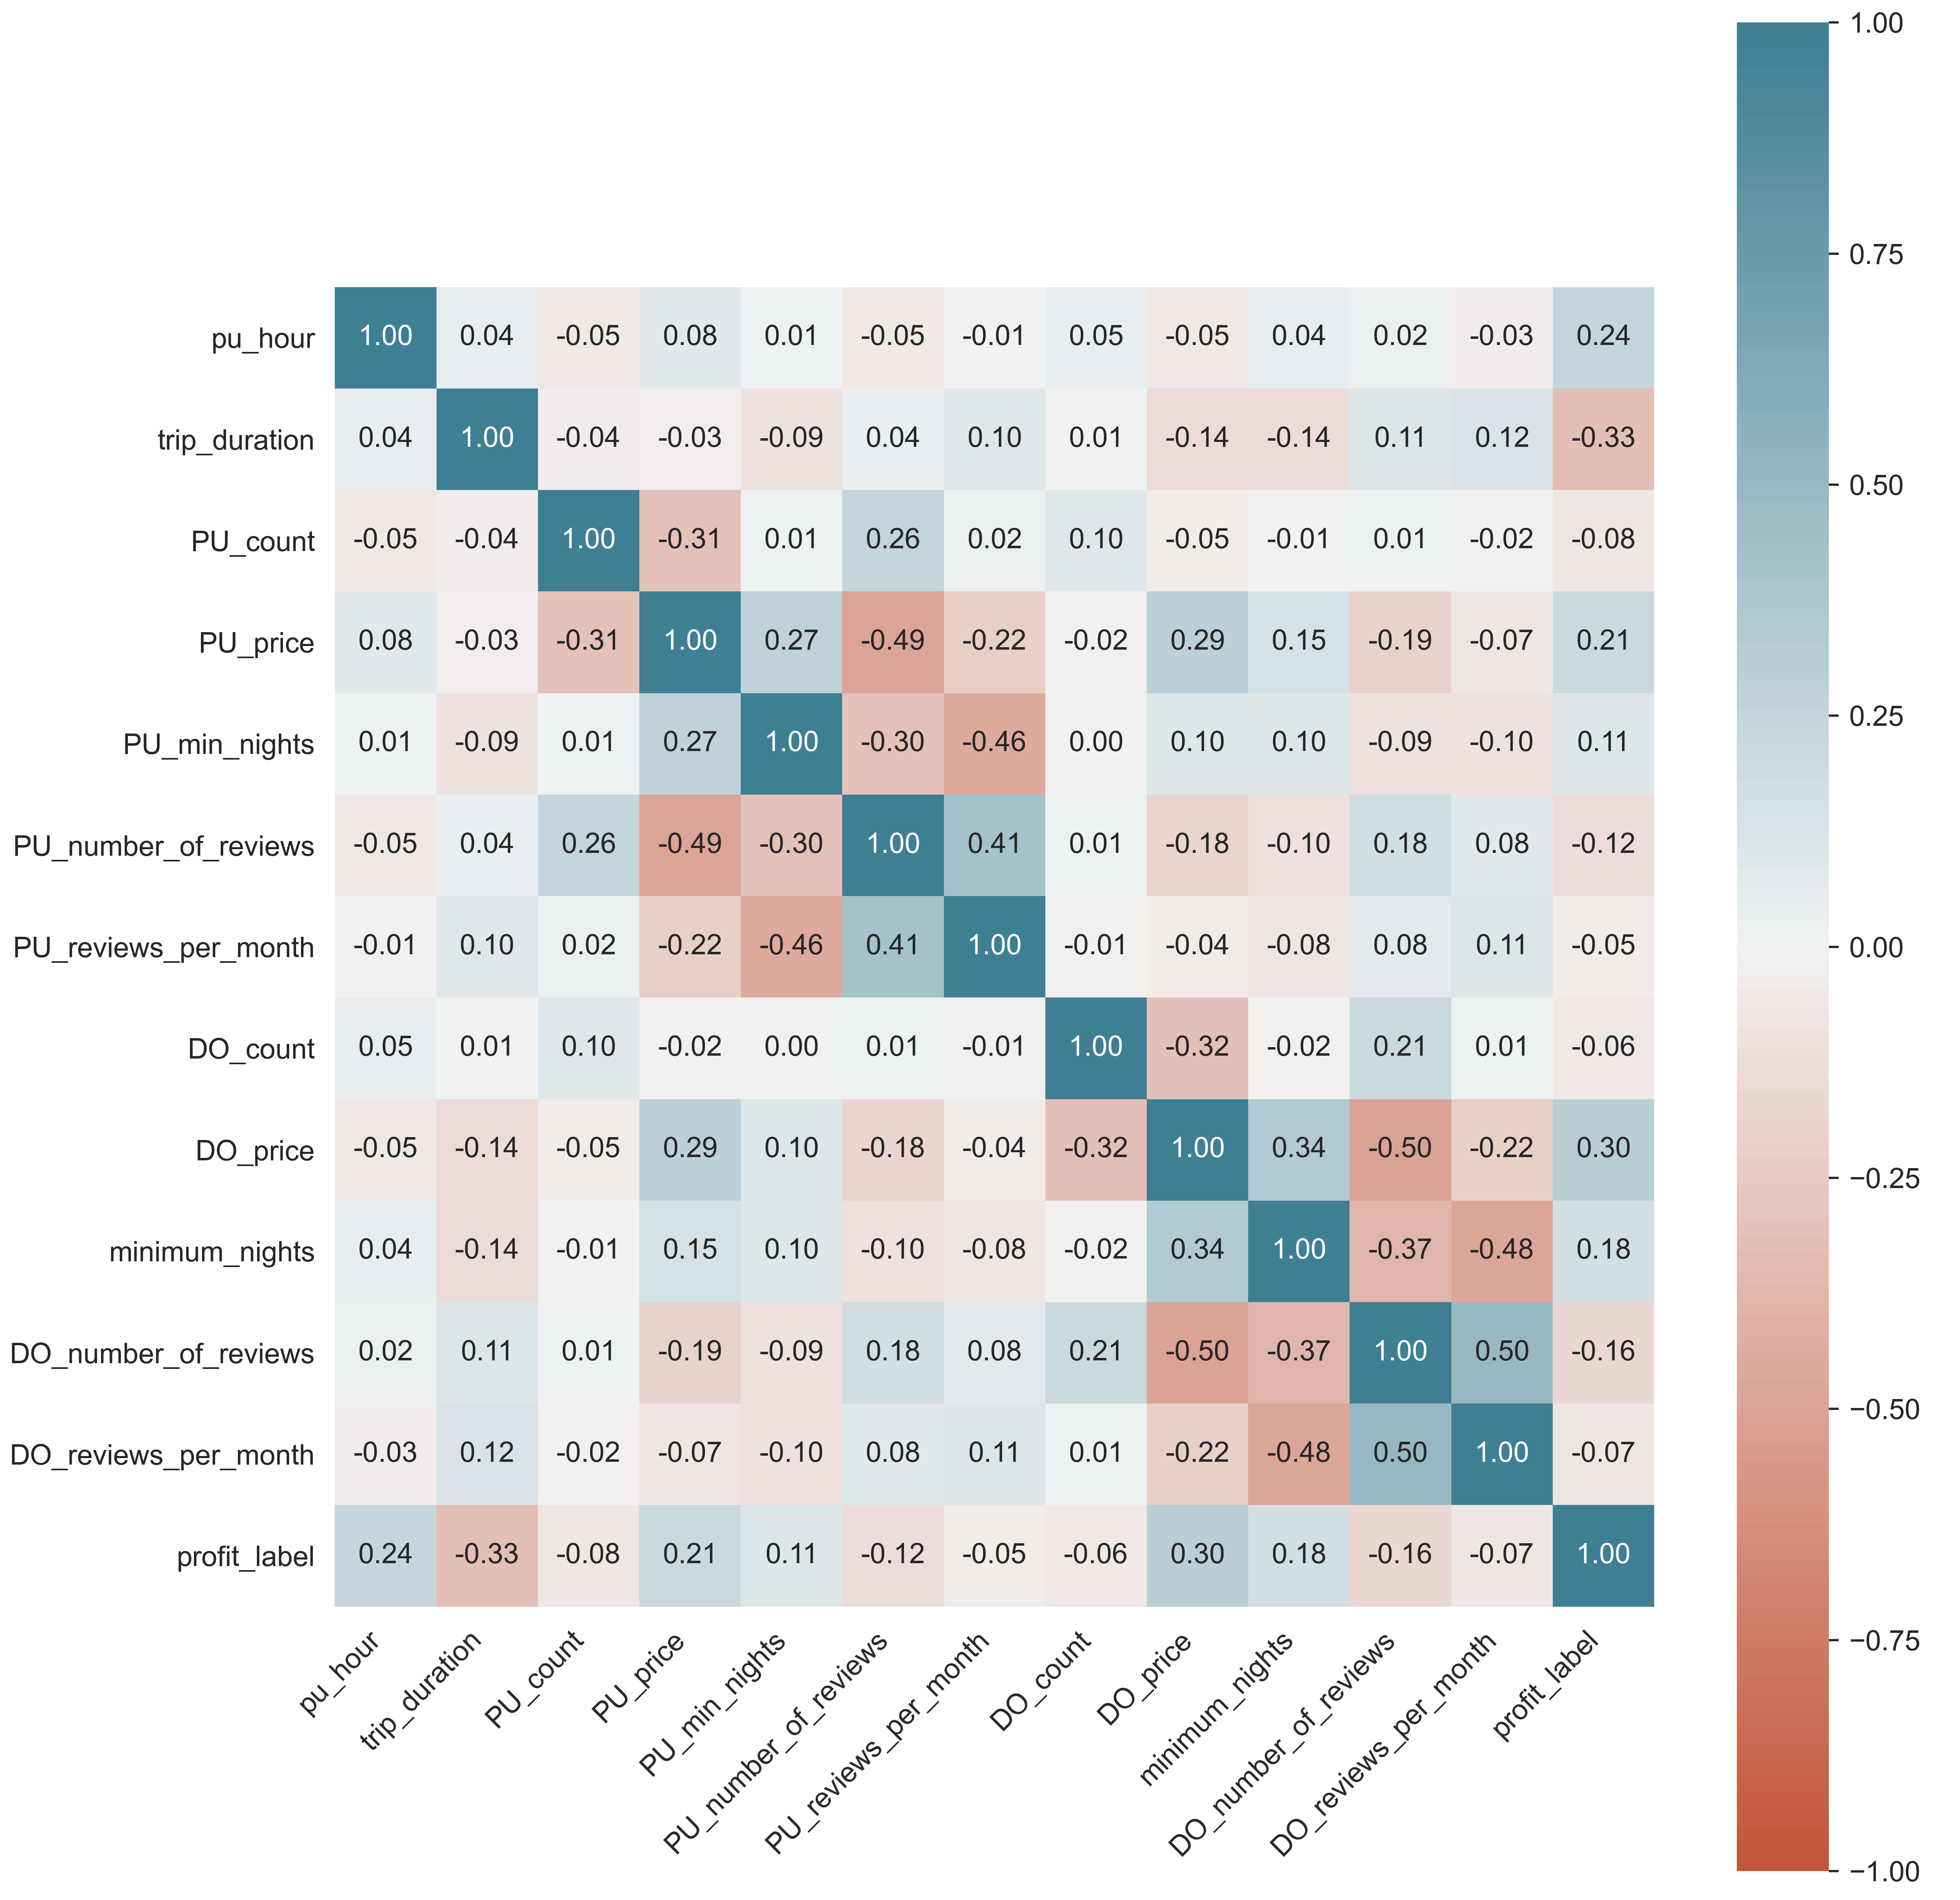
\includegraphics[width=16cm,height=15cm]{plots/correlation.png}
 \caption{Correlation heat map between model attributes (excluding encoded location attributes)}
\end{figure}



\section{Statistical Modelling}
\subsection{Model}

Many different machine learning classification models were considered for this data set. Since the independence of features was not present (see Figure 11), a decision tree classifier was used. A decision tree classifier is also simple to interpret, unlike a Random Forest classifier. The model could be shared easily within taxi drivers, and there would be no need to change the habits of New York Taxi drivers with new technology, they could simply use a tree to make their decision. A decision tree also does not make any assumptions about the data and interaction between variables. To carry out this classification, the following procedure was followed:
\begin{enumerate}
    \item The one hot encoding of attributes \verb|PU_boroughID| and \verb|DO_boroughID| were added to the dataset (and the original attributes removed)
    \item Two data sets were created - a data set comprising of all of the features outlined in section 1.3 (\verb|data_w_airbnb|), and a secondary dataset with only the driving factors (\verb|data_w_o_airbnb|)
    \item These were then split into training and testing sets - May and June were used to predict July
    \item The datasets were scaled, and the components reduced via PCA
\end{enumerate} 
The parameter of the decision tree classifier \verb|max_depth| was then fine-tuned (Figure 13) and the final model was obtained.

\begin{figure}[!htb]
\centering
\begin{minipage}[b]{0.45\linewidth}
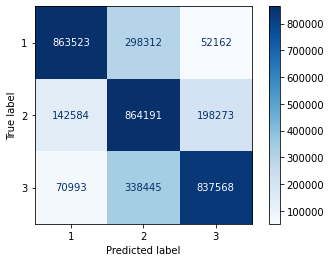
\includegraphics[scale=0.6]{plots/error_matrix.png}
\caption{Confusion matrix for Decision tree with max depth = 15}
\label{fig:minipage1}
\end{minipage}
\hspace{10mm}%   
\quad
\begin{minipage}[b]{0.45\linewidth}
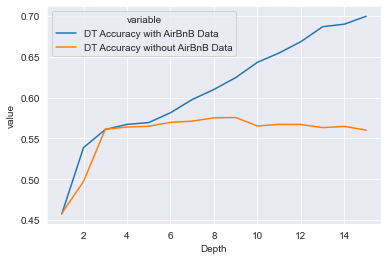
\includegraphics[scale=0.6]{plots/DT_accuracy.png}
\caption{Accuracy of Decision Tree classifier for different values of max depth}
\label{fig:minipage2}
\end{minipage}
\end{figure}


\subsection{Results}
From the cross validation, we obtained a final accuracy score of 70.0\% for the decision tree with AirBnB data, and 56.1\% for the decision tree without. From the confusion matrix, we can see that the classifier had higher precision for low profitability rides (80.2\%) and high profitability rides (77.8\%), over medium profitability rides (57.6\%). The misclassification of high profitability trips as medium is most likely due to uneven geographical spread of high profitability trips. As seen in Figures 7 and 8, the majority of zones have low or medium trips, which may skew our classification. We also see that as \verb|max_depth| in the decision tree increases, the accuracy of the classifier with the AirBnB data increases, whilst the classifier without it plateaus. This is most likely due to the AirBnB classifier having many more features, and so as it gets deeper it can utilise more features, unlike the base classifier.


\subsection{Recommendations}
From the initial analysis, we could see that there existed slight correlation (Figure 11) between the AirBnB data and the profitability of a given taxi ride. Most notably, shorter rides seemed to be very slightly correlated with higher profitability, and higher median listing prices in the drop off zone seemed to slightly correlate with higher trip profitability. These correlations however were not significant enough to greatly enhance profitability classification. As for the model, 70\% accuracy is considered quite good, especially in comparison to the base classifier's 56.1\%. This may be due to having more features than the base model, as a deep decision tree is more suited to datasets with more features. The AirBnB data provides interesting insights into New York's accommodation and transport relationship, as well as improve our model. However, the lack of correlation to a trip's profitability, as well as only providing our classifier with 70\% accuracy, means that the data may not be worth purchasing for Taxi drivers and companies. It could definitely be used to create a more thorough model when combined with numerous other sources of data.

\subsection{Conclusion}
A given taxi ride's profitability can be affected by numerous external factors. Time of pick up, the duration of the trip and the pickup/drop off locations are all important in determining how profitable a trip is. To help classify a trip's profitability, the data was augmented from AirBnB house listing data. Although this data improved our profitability predictions, it is recommended that this data is not purchased, as it may be just as useful to find extra predictors which are available at no cost.


\clearpage

% BEGIN REFERENCES SECTION
% You may change this to use bibtex, but this is also fine if you are unsure how to do it.
% You may use \href{} or \url{} to create hyperlinks if you wish.
\begin{thebibliography}{1}
\setlength{\parfillskip}{0pt plus 1fil}
\bibitem{open_data_website}
City of New York, NYC Open Data. (2017). NYC Open Data. NYC Open Data.\\ https://opendata.cityofnewyork.us/projects/

\bibitem{taxi_demand}
Correa, D., Xie, K., \& Ozbay, K. (2017, January). Exploring the taxi and Uber demand in New York City: An empirical analysis and spatial modeling. In 96th Annual Meeting of the Transportation Research Board, Washington, DC.

\bibitem{taxi_supply}
Kamga, C., Yazici, M. A., \& Singhal, A. (2015). Analysis of taxi demand and supply in New York City: implications of recent taxi regulations. Transportation Planning and Technology, 38(6), 601-625.

\bibitem{taxi_revenue}
Dong, Y., Zhang, Z., Fu, R., \& Xie, N. (2016, June). Revealing New York taxi drivers' operation patterns focusing on the revenue aspect. In 2016 12th World Congress on Intelligent Control and Automation (WCICA) (pp. 1052-1057). IEEE.

\bibitem{airbnb_data}
Inside Airbnb. Adding data to the debate. (2019). Inside Airbnb. http://insideairbnb.com/get-the-data.html
\bibitem{taxi_data}
New York Taxi and Limousine Commission. (2019). TLC Trip Record Data - TLC. TLC Trip Record Data. https://www1.nyc.gov/site/tlc/about/tlc-trip-record-data.page
\bibitem{tourism_data}
Office of the New York State Comptroller. (2021, April). The Tourism Industry in New York City. https://www.osc.state.ny.us/reports/osdc/tourism-industry-new-york-city
\bibitem{geo_data}
NYC Taxi Zones. (2021). NYC Open Data.
https://data.cityofnewyork.us/Transportation/NYC-Taxi-Zones
\bibitem{IRS}
Standard Mileage Rates | Internal Revenue Service. (2021, March 17). Internal Revenue Service. https://www.irs.gov/tax-professionals/standard-mileage-rates
\bibitem{taxi_fare}
Taxi Fare - TLC. (2021). Taxi and Limousine Commission.
https://www1.nyc.gov/site/tlc/passengers/taxi-fare.page

\end{thebibliography}
\end{document}